
\section{Theoretical Fundamentals}

\subsection{Waterfall Model}
The Waterfall model is a sequential model for software projects development. It is a sequential model and its name is given because of how the different phases follow one another.

\begin{figure}[!h]
	\center
	\label{figure3}
	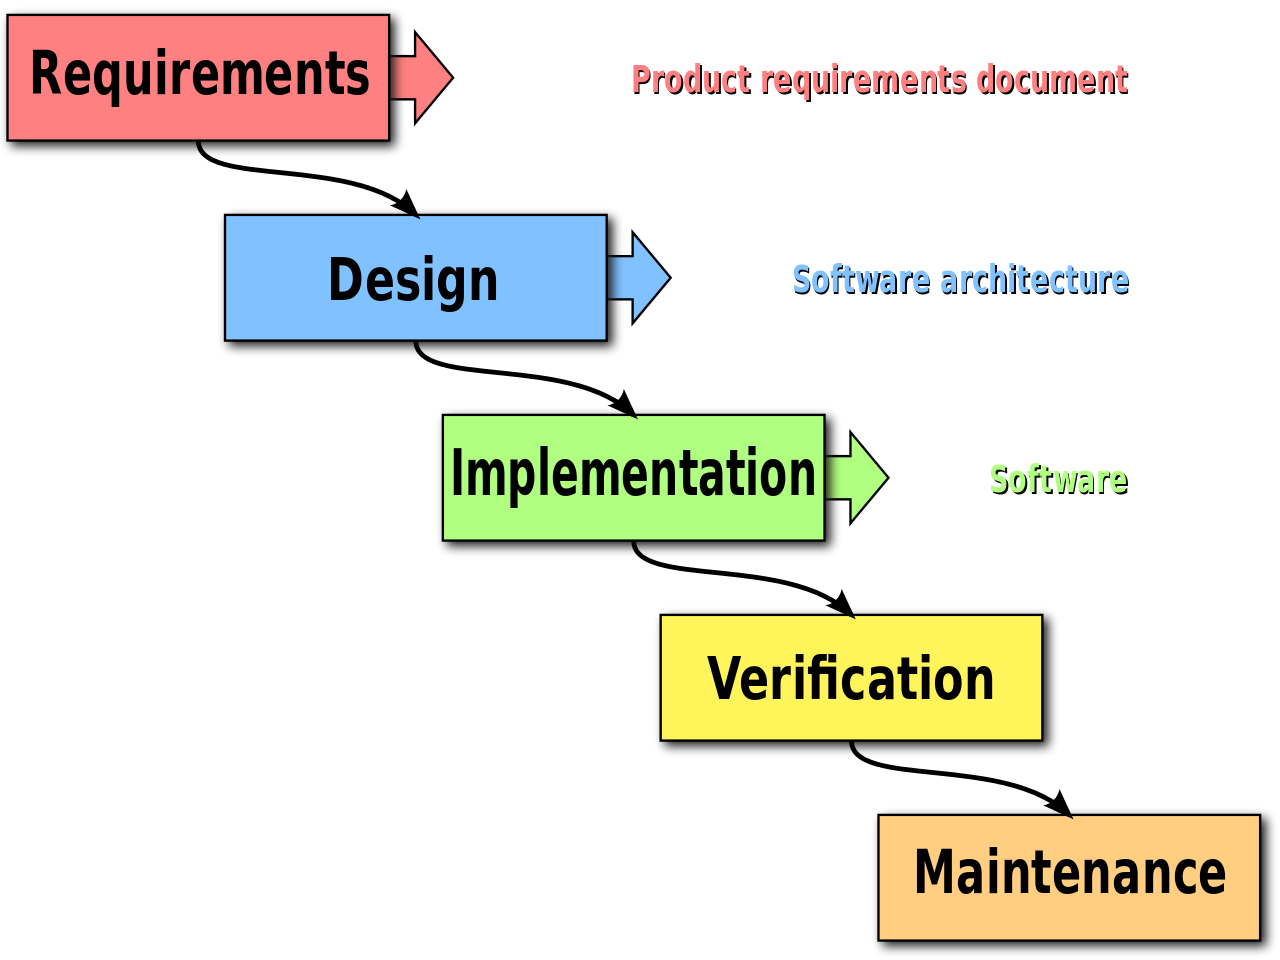
\includegraphics[scale=0.30]{Figures/waterfall} \\
	\caption {Waterfall Model}
\end{figure}

\noindent \textbf{Analysis Phase}: Execution of models and diagrams that explain the problem and its solution. It normally explains what is the problem to be solved, the requirements and constraints to solve it, as well as a brief and general hardware/software specification. It is also in this phase that a division of member’s tasks is made with also the deadlines for each different stage of the project. \\[\baselineskip]
%\newpage
\textbf{Design Phase}: A more in-depth Hardware/Software specification. In this phase, there needs to be a more scientific explanation of the problem and the solutions that will solve it.\\[\baselineskip]
\textbf{Implementation Phase}: Creation of a final prototype that solves the initial problem.\\[\baselineskip]
\textbf{Verification Phase}: Testing the final prototype in all the different situations that the product may face and do the needed changes so the final product passes those tests.\\[\baselineskip]
\textbf{Maintenance Phase}: Support and maintenance of the final product.\\[\baselineskip]
\indent In all the stages of the project a verification of the last phase should be done, before starting the following phase of the project.\\
\indent Despite being a sequential model, the Waterfall Model allows the return to earlier
phases of the project to correct mistakes that were only noticed ahead or, for example, some specification was poorly made, being possible correcting the mistakes before moving forward.

\subsection{Hypervisor}
Layer of software that allows to run several independent execution environments in a single
computer\\
\indent The bare-metal hypervisors run directly on the native hardware\\
\indent Virtualizing the critical hardware devices to create several isolated partitions

\begin{figure}[!h]
	\center
	\label{figure6}
	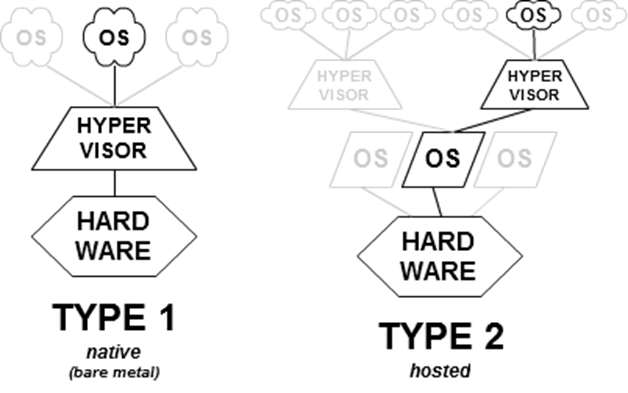
\includegraphics[scale=0.65]{Figures/Hypervisor} \\
	\caption {Hypervisor}
\end{figure}
